\documentclass[12pt, a4paper]{article}
\usepackage[T1]{fontenc}
\usepackage{lmodern}
\usepackage[portuguese]{babel}
\usepackage{graphicx}
\usepackage{geometry}
\usepackage{amsmath}
\usepackage{booktabs} % For better-looking tables
\usepackage{siunitx} % For proper number formatting
\usepackage{float} % For controlling figure placement
\usepackage{threeparttable}
\usepackage{booktabs}

\geometry{
 a4paper,
 left=3cm,
 top=2cm,
 right=2cm,
 bottom=2cm
}

\begin{document}

\begin{center}
    \textbf{\large UNIVERSIDADE FEDERAL DO RIO GRANDE DO SUL} \\
    \textbf{\large INSTITUTO DE FÍSICA} \\
    \vspace{3cm}
    \textbf{\Large CADERNO DE LABORATÓRIO 3} \\
    \vspace{1cm}
    \textbf{\large MEDINDO CAMPOS MAGNÉTICOS} \\
    \vspace{3cm}
    
    \begin{tabular}{rl}
        \textbf{Integrantes:} & Guilherme Franke Riter - 00579589 \\
                               & Júlia Matzenbacher Henicka Germano - 00579271 \\
                               & Leonardo Kawai Suarez - 00578511 \\
                               & Leonardo Werner Morel Dias - 00590887 \\
    \end{tabular}
    
    \vspace{12cm}
    \textbf{\large Porto Alegre, RS} \\
    \textbf{\large 4 de junho de 2025} \\
\end{center}\newpage

\subsection*{Parâmetros Experimentais}

O objetivo do experimento é verificar a relação entre o campo magnético gerado por uma bobina e a distância do ponto de medição. Para isso, calculamos o campo magnético da bobina a partir de medidas de deflexão de uma bússola e do campo magnético horizontal terrestre em Porto Alegre, que é de aproximadamente $B_{\text{hor}}^{T} = \SI{16.555}{\micro\tesla}$ e utilizamos a relação \[B_{bob}=B_{hor}^T\tan\theta,\] onde $\theta$ é o ângulo de deflexão da bússola.

Mantivemos constantes o número de espiras ($N$), o material do núcleo da bobina e a corrente ($I$), variando apenas a distância ($d$) entre a bobina e a bússola. Dessa forma, supomos que o campo magnético da bobina é dado por uma expressão do tipo \[B_{bob} = Kd^n,\] onde $K$ é uma constante e $n$ é um expoente que indica a potência da relação entre o campo magnético e a distância do ponto de medição. 

A seguir, apresentamos os parâmetros do experimento:
    \begin{table}[H]
        \centering
        \caption{Parâmetros do experimento de medição de campos magnéticos}
        \label{tab:parametros_experimento}
        \begin{tabular}{ll}
        \toprule
        \textbf{Parâmetro} \\
        \midrule
        Número de espiras ($N$) & 1000 \\
        Material do núcleo da bobina & Ar \\
        Corrente ($I$) & $127$ mA \\
        Intervalo de distâncias ($d$) & $[0.06, 0.3]$ m \\
        $B_{\text{hor}}^{T}$ & $\SI{16.555}{\micro\tesla}$\\
        \bottomrule
        \end{tabular}
    \end{table}

\subsection*{Dados Coletados}

Primeiro, a partir das medidas de deflexão da bússola, calculamos o campo magnético da bobina em função da distância. Os dados coletados foram os seguintes:

    \begin{figure}[H]
        \centering
        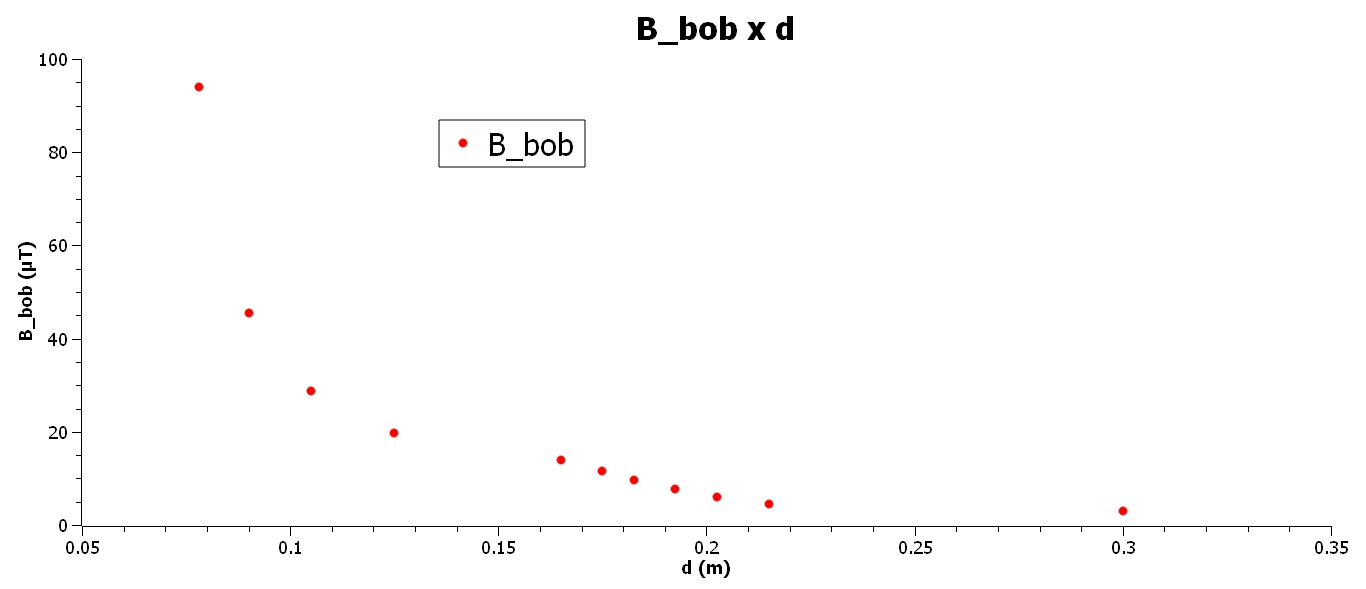
\includegraphics[width=\textwidth]{grafico-lab3-dados.jpeg}
        \caption{Dados coletados no experimento de medição de campos magnéticos.}
        \label{fig:dados_experimentais}
    \end{figure}

\subsection*{Ajuste no intervalo completo de distâncias}

Posteriormente, fizemos uma linearização dos dados, utilizando a relação \[B_{bob} = Kd^n\] para obter uma função do tipo \[\ln(B_{bob}) = \ln(K) + n \cdot \ln(d).\] Assim, dada a equação do ajuste linear \[y = A \cdot x + B,\] podemos identificar que $A = n$ e $B = \ln(K)$, ou $K=e^B$.

    \begin{figure}[H]
        \centering
        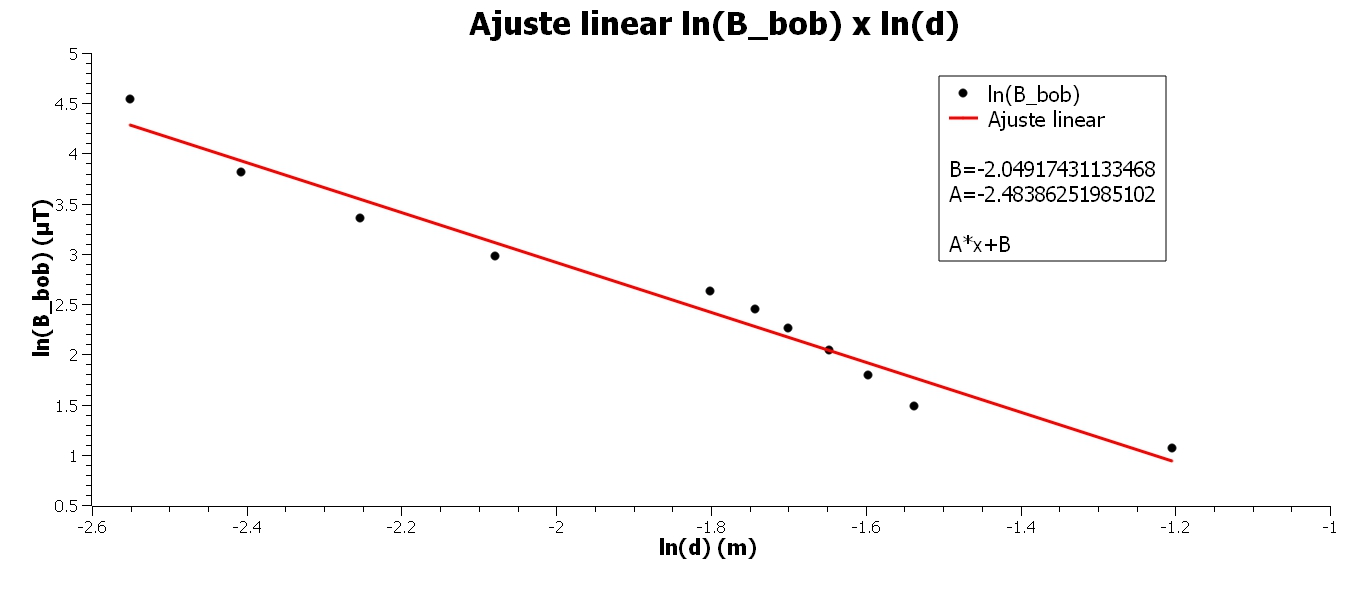
\includegraphics[width=\textwidth]{grafico-lab3-ajuste.jpeg}
        \caption{Ajuste dos dados experimentais.}
        \label{fig:ajuste_dados}
    \end{figure}

    \begin{table}[h]
        \centering
        \caption{Resultado do ajuste linear dos dados experimentais.}
        \label{tab:ajuste_dados}
        \begin{tabular}{lc}
        \toprule
        Função do ajuste & $A \cdot x + B$ \\
        Intervalo & [\num{-2.55104645229255}, \num{-1.20397280432594}] \\
        Coeficiente da reta ($A$) & \num{-2.48386251985102} $\pm$ \num{0.145909020050064} \\
        Intercepto-Y ($B$) & \num{-2.04917431133468} $\pm$ \num{0.278116198800418} \\
        \midrule
        $\chi^2$ & \num{0.320341492396555} \\
        $R^2$ & \num{0.996193283189016} \\
        \bottomrule
        \end{tabular}
        \smallskip
        \begin{tablenotes}
            \item[a] O coeficiente de determinação ($R^2$) $\approx0.996$ indica um excelente ajuste aos dados.
        \end{tablenotes}
    \end{table}

    Dos dados Tabela 2, podemos escrever a equação do ajuste linear como \[\ln(B_{bob}) = \num{-2.48386251985102} \cdot \ln(d) + \num{-2.04917431133468}.\] Ou, na relação que supomos inicialmente, temos que \[B_{bob} = \num{0.129} \cdot d^{-2.484}.\]

\subsection*{Ajuste no intervalo de distâncias mais distantes}
    
    No entanto, podemos restringir o intervalo de distâncias para considerar apenas os pontos mais distantes, onde a relação entre o campo magnético e a distância é mais linear. Para isso, consideramos o intervalo $[0.15, 0.3]$ m, que corresponde aos pontos mais distantes do experimento.

    \begin{figure}[H]
        \centering
        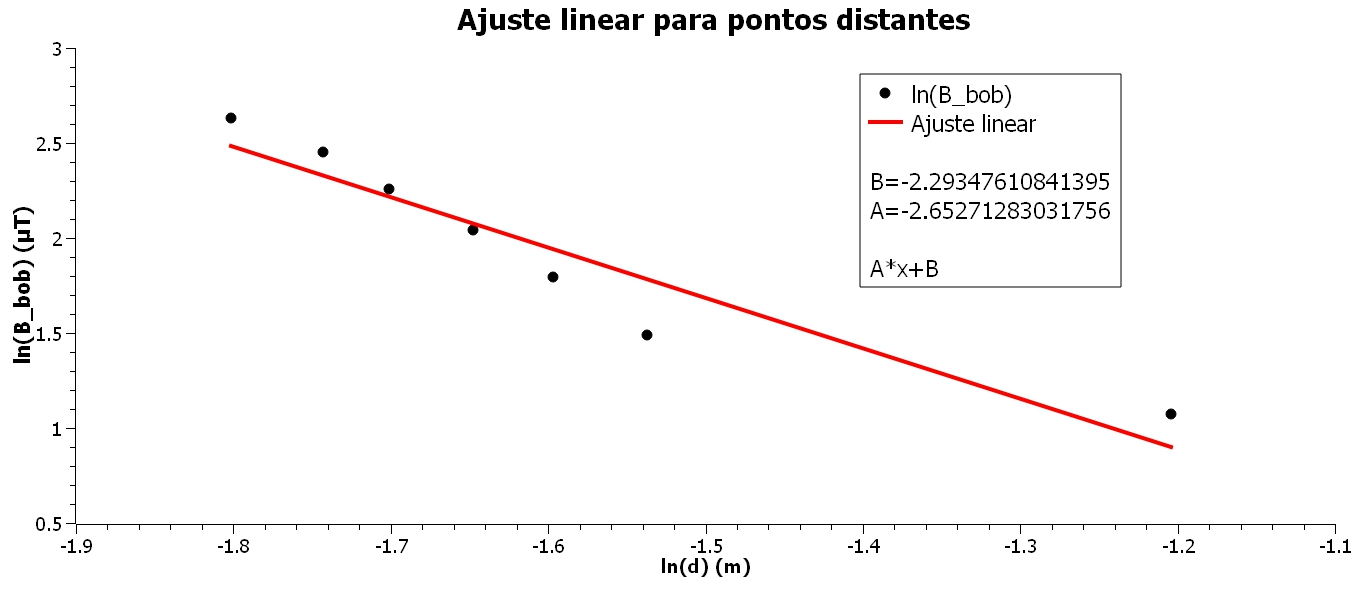
\includegraphics[width=\textwidth]{grafico-lab3-ajuste-distante.jpeg}
        \caption{Ajuste dos dados experimentais considerando apenas pontos distantes.}
        \label{fig:ajuste_dados_distante}
    \end{figure}

    \begin{table}[h]
        \centering
        \caption{Resultados do ajuste linear para pontos distantes.}
        \label{tab:ajuste_completo}
        \begin{tabular}{lc}
        \toprule
        Função do ajuste & $A \cdot x + B$ \\
        Intervalo & [\num{-1.80180980508156}, \num{-1.20397280432594}] \\
        Coeficiente da reta ($A$) & \num{-2.65271283031756} $\pm$ \num{0.38709713608572} \\
        Intercepto-Y ($B$) & \num{-2.29347610841395} $\pm$ \num{0.62512459619061} \\
        $\chi^2$ & \num{0.175541978508799} \\
        $R^2$ & \num{0.993903293483138} \\
        \bottomrule
        \end{tabular}
        \smallskip
        \begin{tablenotes}
            \item[a] O coeficiente de determinação ($R^2$) $\approx0.993$ indica um bom ajuste aos dados (obs.: a razão para o valor de $R^2$ ser menor que o do ajuste completo pode ser o último ponto, que é um pouco mais distante do que os demais; contudo, quando este ponto fora removido, o valor de $n$ ultrapassava $-4$, o que difere da relação esperada de $d\approx-3$).
        \end{tablenotes}
    \end{table}

    A equação do ajuste linear para os pontos distantes é \[\ln(B_{bob}) = \num{-2.65271283031756} \cdot \ln(d) + \num{-2.29347610841395}.\] Ou então, \[B_{bob} = \num{0.101} \cdot d^{-2.653},\] o que verifica a proporção \(B \propto d^{-3}\) para pontos distantes da bobina.

\end{document}